\documentclass[]{beamer}

%Package declarations
\usepackage[utf8]{inputenc}
\usepackage[spanish]{babel}
\usepackage{natbib}
\usepackage{graphicx}

%Theme related configurations
\usecolortheme{seahorse}
\usetheme{Berkeley}

% \graphicspath{..\Docs}



%Title of the presentation
\title{Instrumentación electrónica avanzada cómo oportunidad para la automatización de sistemas de producción de alimentos en áreas del corredor seco.}
\author{Luis Guillermo García Ordóñez}
\date{10 de Noviembre 2018}



\begin{document}
\maketitle
\section{¿Qué es el corredor seco?}

\begin{frame}{¿Qué es el corredor seco?}

\note{Desde un punto de vista ecológico}
Es una zona de bosque tropical seco que presenta un patrón de lluvias irregulares, caracterizado por extensos períodos de sequías reduciéndose hasta 30\% y 40\% durante el período del niño.
\begin{figure}
    \centering
    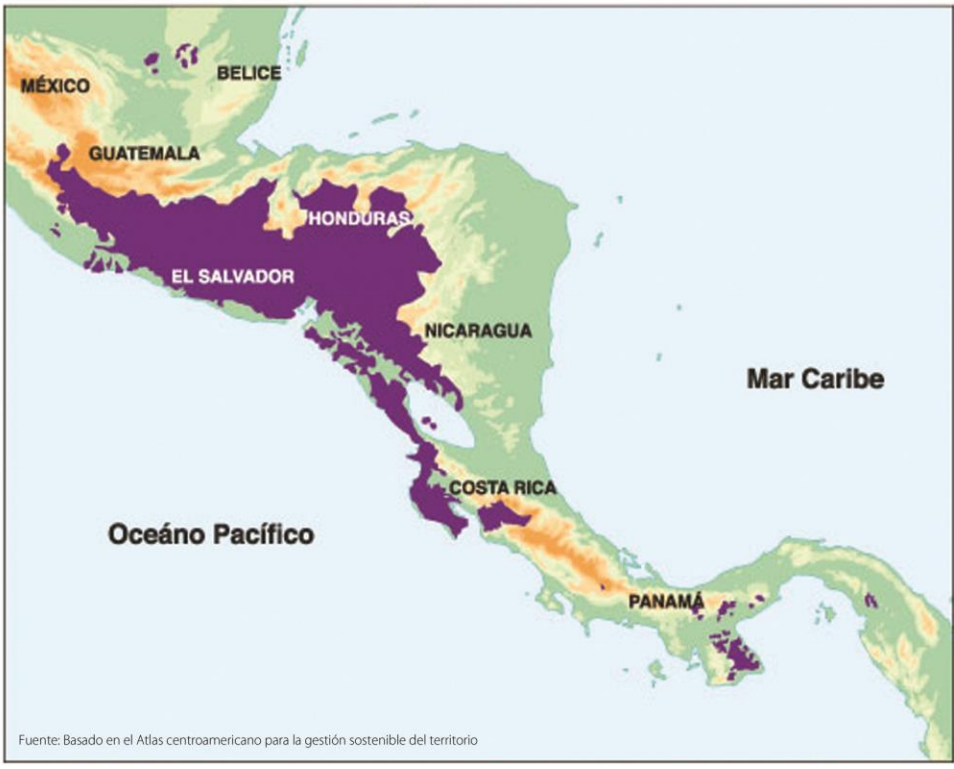
\includegraphics[width=0.5\textwidth]{Docs/Mapa_CS}
    \caption{\small \textit{Dry Corridor Central America}, Situation Report, June 2016, \textbf{FAO}}
    \label{fig:my_label}
\end{figure}
\end{frame}

\begin{frame}{}
\begin{figure}
    \centering
    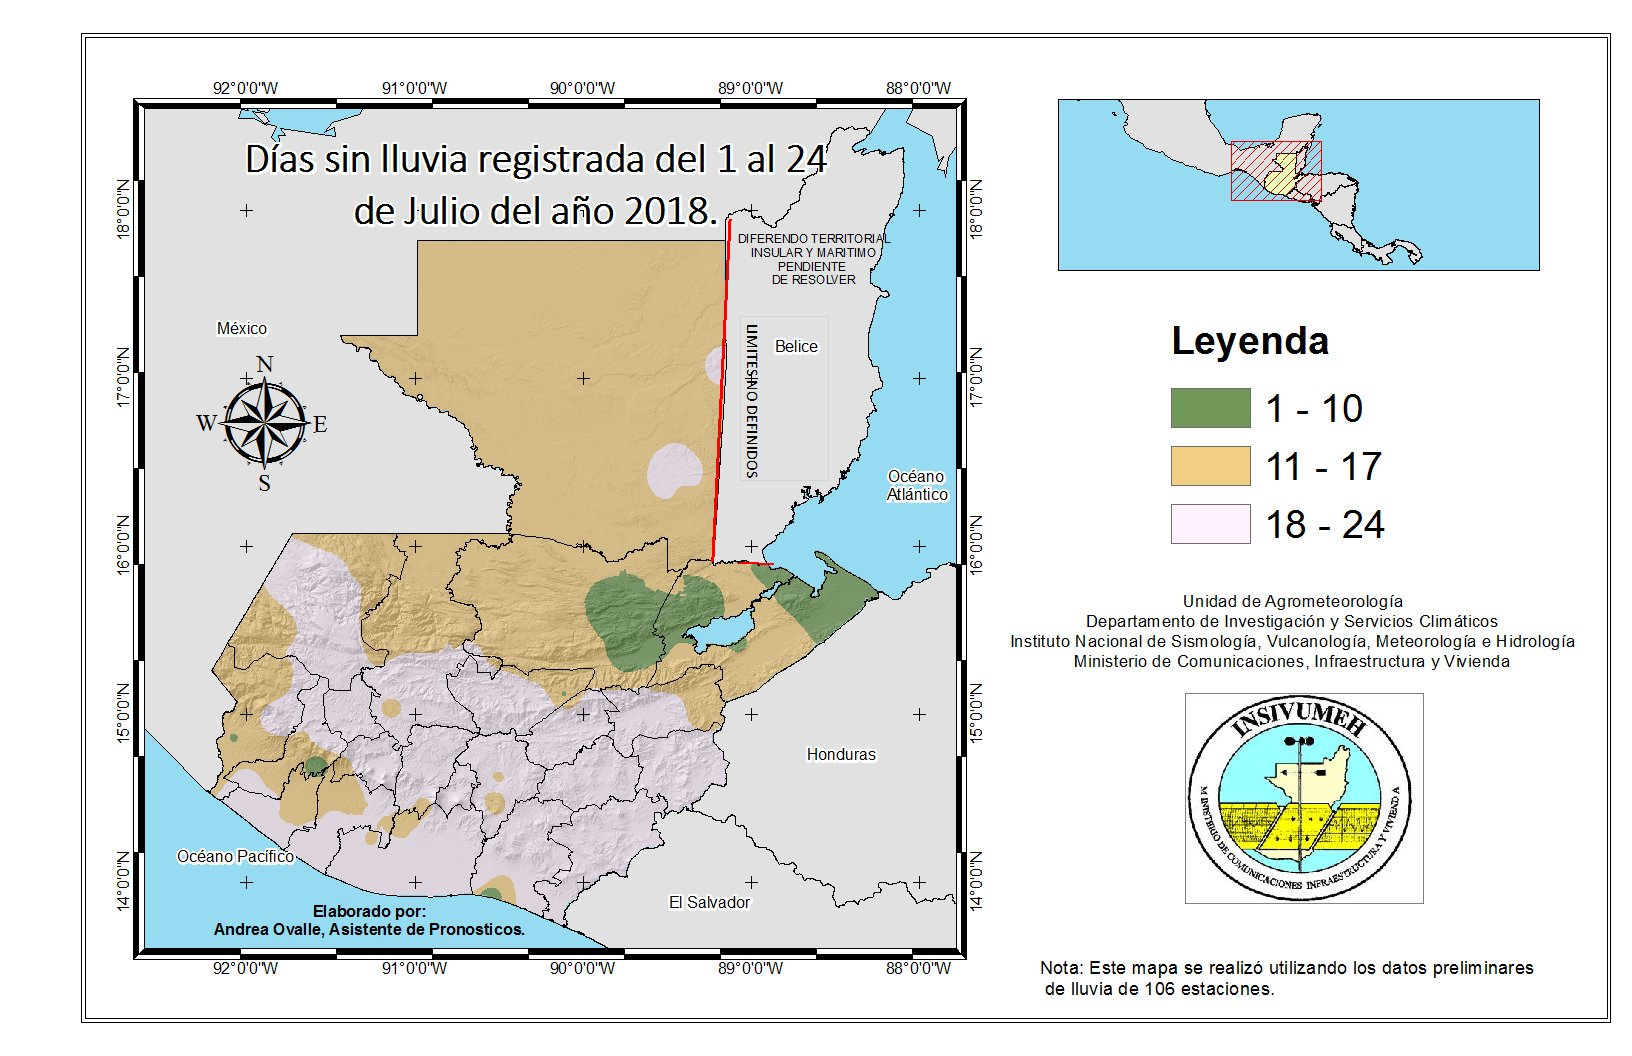
\includegraphics[width=0.9\textwidth]{Docs/diassinlluvia}
    % \caption{Caption}
    \label{fig:my_label}
\end{figure}
\end{frame}

\begin{frame}{La crísis en números}
    \begin{figure}
        \centering
        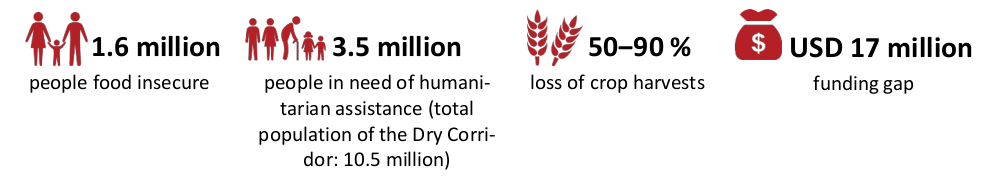
\includegraphics[width=0.8\textwidth]{Docs/cs_in_numbers}
        \caption{Cífras estimadas en centroamérica;  FAO, \textit{Situation Report}, Junio 2016}
        \label{fig:my_label}
    \end{figure}
    \begin{itemize}
      \item Durante la época de lluvias, la primera temporada de producción de maíz y frijol contribuye en 60 y 35 porciento, respectivamente, a la producción total anual.
      \item 1.5 millones de personas necesitan ayuda humanitaria en el 2016. %FAO Situation Report 2016
      \item 175,126 hectáreas de cultivo (maíz, frijol) perdídas en el 2018. %FAO GIEWS UPDATE
      \item 1,290,785 Personas afectadas en Guatemala. %FAO GIEWS UPDATE
    \end{itemize}
\end{frame}

\begin{frame}{¿Cómo mitigar este problema?}{La respuesta de la FAO en el 2016}
      \begin{itemize}
        \item Implementación de un sistema de emergencia  para beneficio de 7000 famililas.
        \item Creación de un fondo de emergencia y actividades de rehabilitación (SFERA) exclusivo para el corredor seco.
        \item Implementación de un programa de respuesta para fortalecer las capacidades de manejo de riesgo a nivel nacional promoviendo buenas prácticas y \textbf{nuevas tecnologías}, reduciendo el impacto del clíma extremo.
      \end{itemize}

\end{frame}

\begin{frame}{¿Qué nos espera?}{Algunos escenearios para el 2030}
  \begin{figure}
     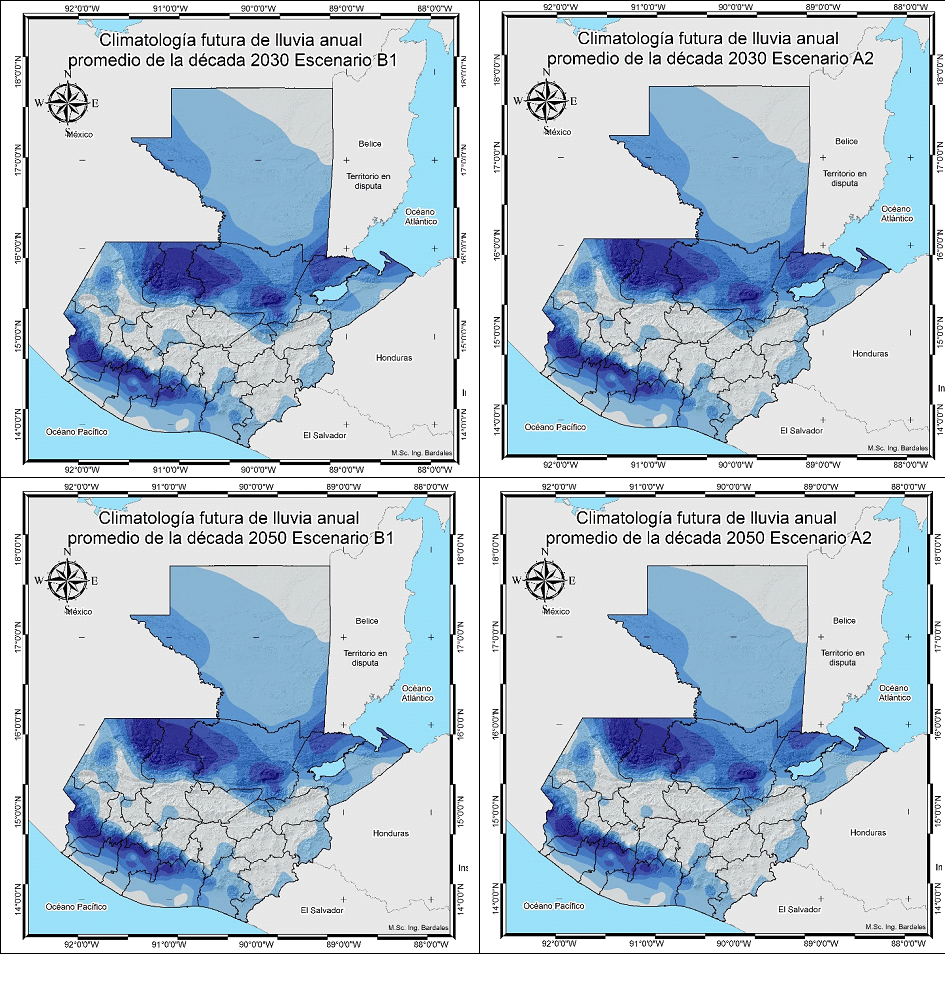
\includegraphics[width=0.6\textwidth]{Docs/Predictions}
    \caption{Presipitación promedio anual estimada para el 2030 según distintos modelos \emph{Fuente: INSIVUMEH}}
    \label{Fig:Lluvias2050}
  \end{figure}
\end{frame}

\section{La Electrónica como posible solución}
\subsection{Electrónica Aplicada a la agricultura}

\begin{frame}{La electrónica como posible solución}
  \begin{figure}
    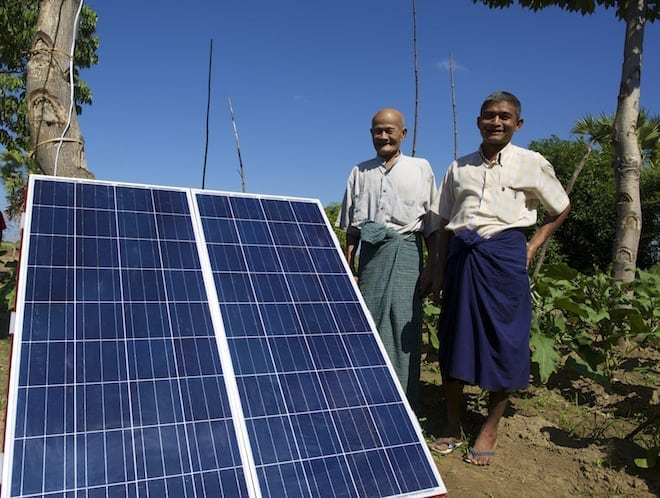
\includegraphics[width=0.9\textwidth]{Docs/lotus-solar-pump}
  \end{figure}
\end{frame}

\begin{frame}{Antes de empezar!!!!}{El elefante en la habitación.}
  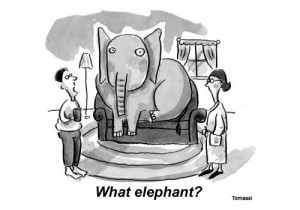
\includegraphics{Docs/elefant_in_room}
\end{frame}

\begin{frame}{Antes de empezar!!!!}{El elefante en la habitación.}
  \textbf{¿Cómo puede un agricultor adoptar estas tecnologías?}
  Tomando en consideración:
  \begin{itemize}
    \item El precio de esta tecnología.
    \item La curva de aprendizaje
    \item Falta de infraestructura para aplicarlas (La electricidad es parte importante de un componente electrónico....)
  \end{itemize}
\end{frame}

\begin{frame}{¿Cuanto cuesta en realidad?}{La ley de Moore sigue vigente.}
  \begin{figure}
    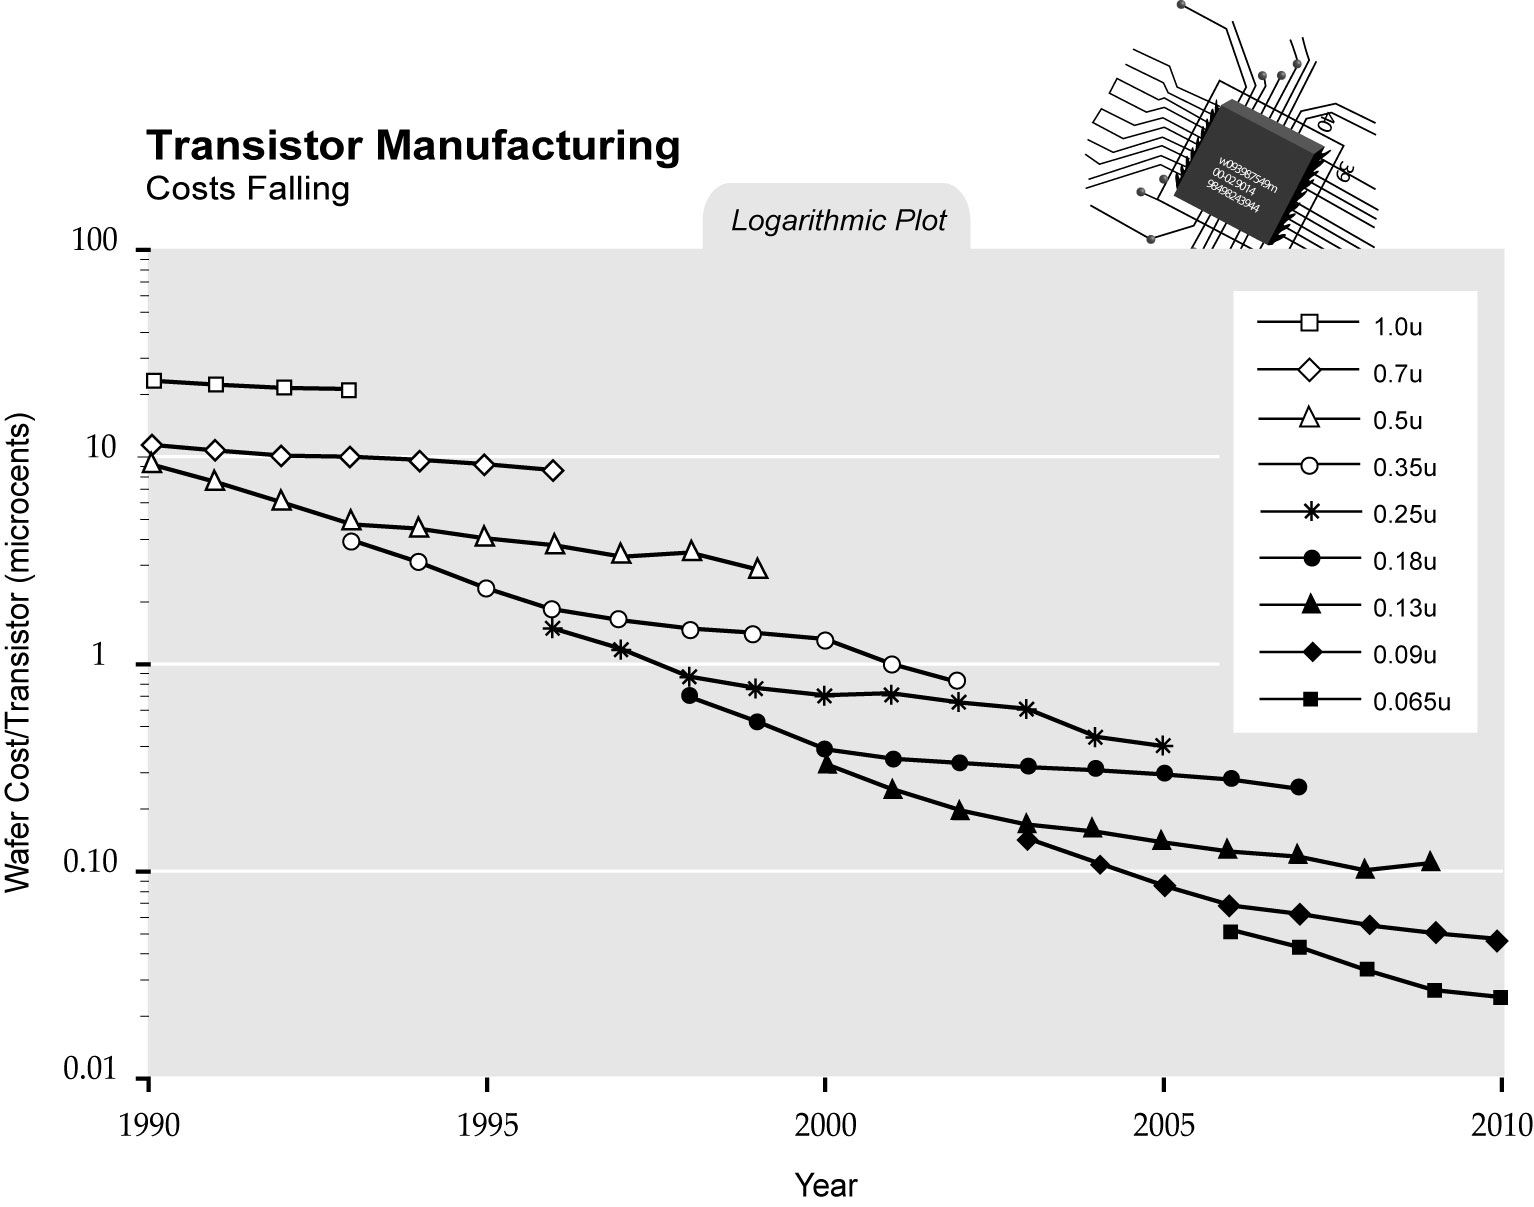
\includegraphics[width=0.8\textwidth]{Docs/Trans_price}
    \caption{\tiny Randall Goodall, D. Fandel, and H.Huff, “Long-Term Productivity Mechanisms of the Semiconductor Industry,” Ninth International Symposium on Silicon Materials Science and Technology, }
    \label{Moore_law}
  \end{figure}
\end{frame}

\begin{frame}
    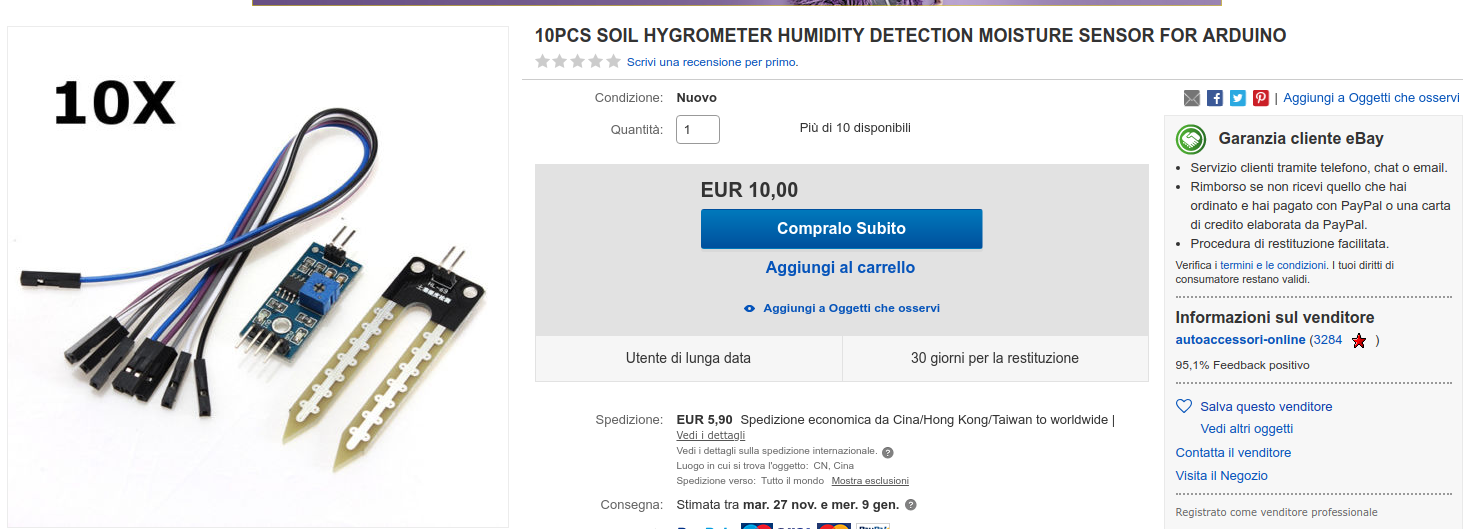
\includegraphics[width=\textwidth]{Docs/soil_humidity}
\end{frame}

\begin{frame}{No es tan difícil}{Si está bien diseñado}
  \begin{columns}
    \begin{column}{0.5\textwidth}
      \center
      \textbf{Curva de aprendizaje del programador:}

      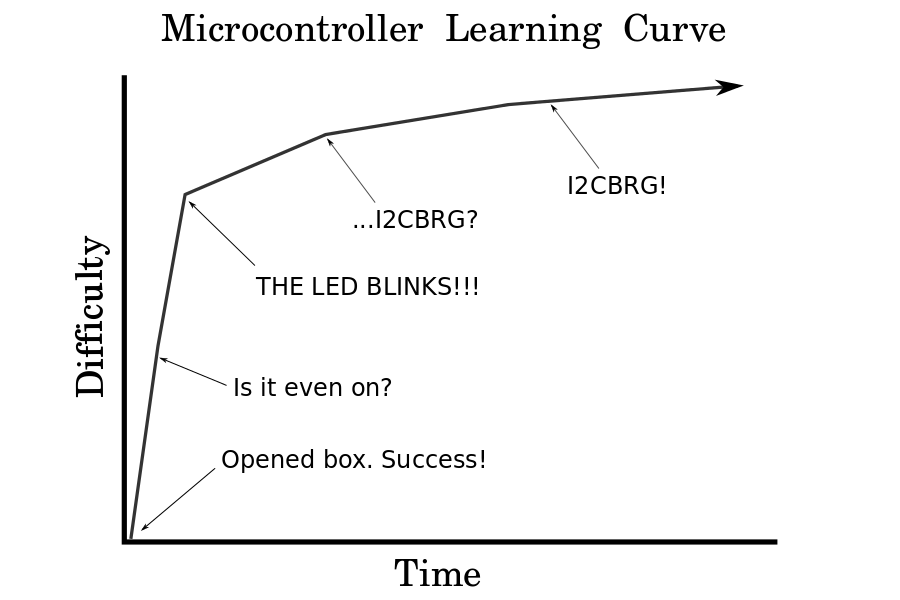
\includegraphics[width=\textwidth]{Docs/micro_lc}
    \end{column}
    \begin{column}{0.5\textwidth}
      \center
      \textbf{Curva de aprendizaje del usuario:}

      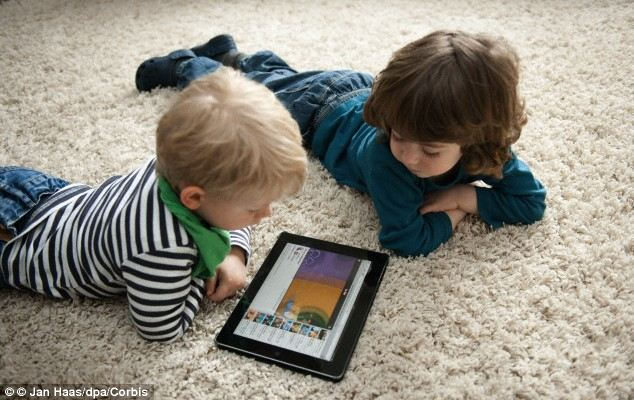
\includegraphics[width=\textwidth]{Docs/baby_tablet}
    \end{column}
\end{columns}
\end{frame}

\begin{frame}{}
  \begin{columns}
    \begin{column}{0.7\textwidth}
      \begin{figure}
        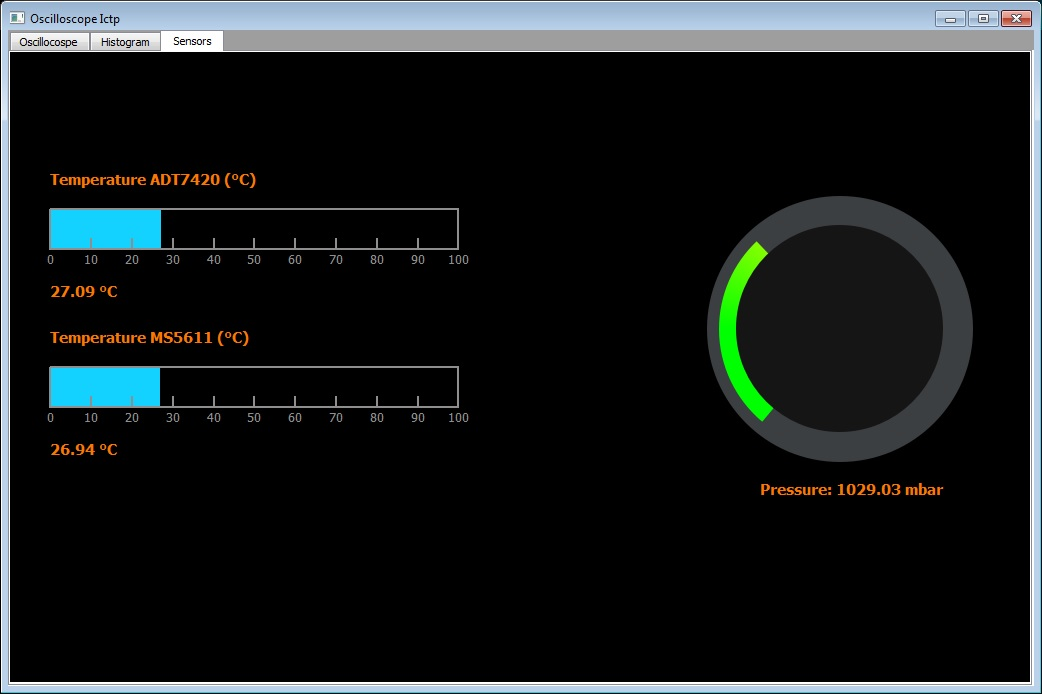
\includegraphics[width=\textwidth]{Docs/sensorfinal}
        \caption{Interfáz gráfica realizada en PyQT para interacción con sensores}
        \label{}
      \end{figure}
    \end{column}
    \begin{column}{0.3\textwidth}
      \begin{figure}
        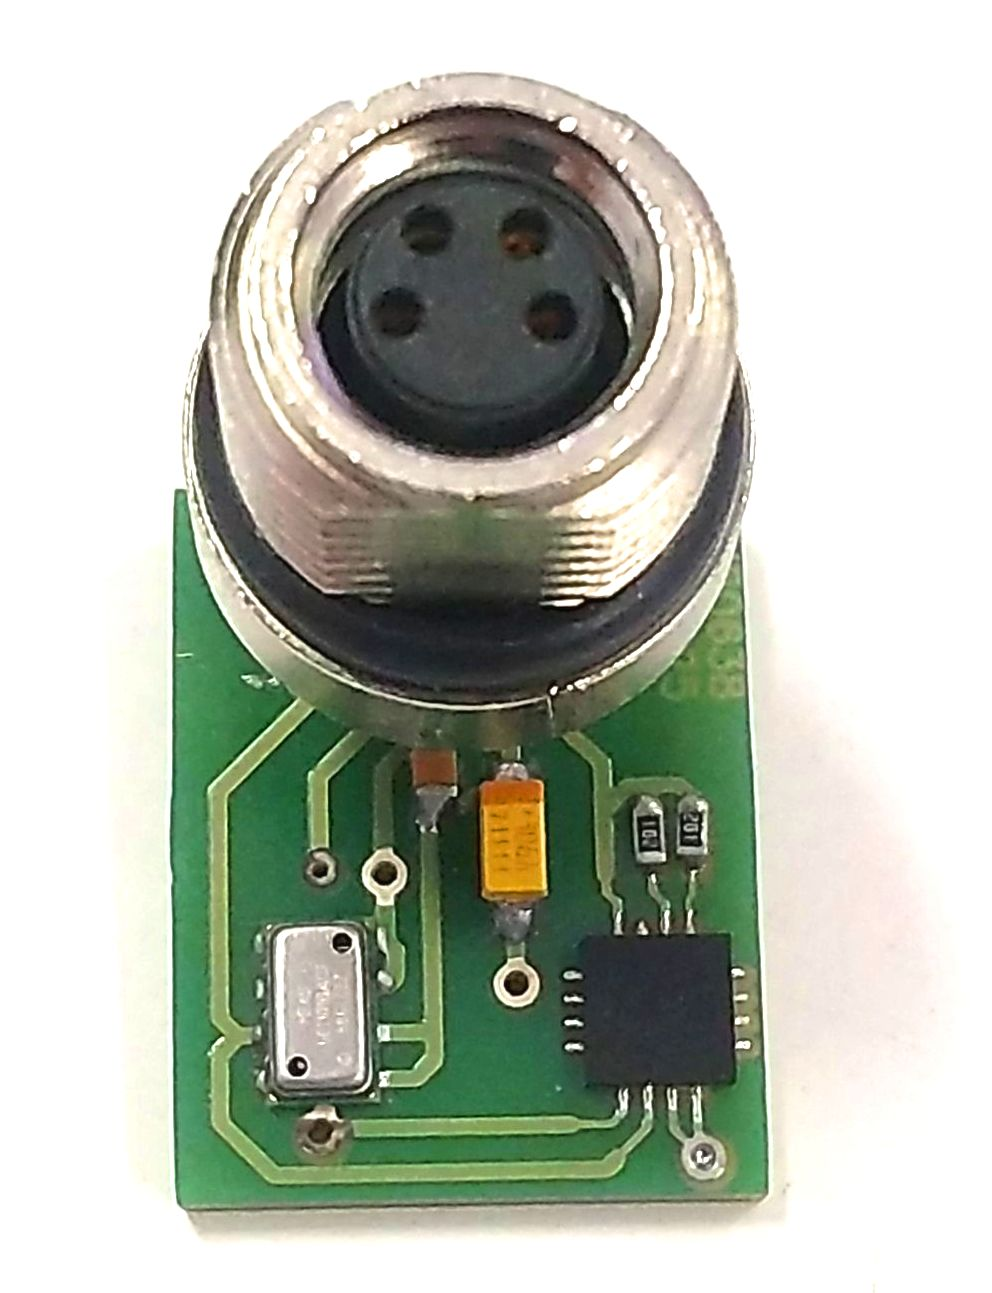
\includegraphics[width=\textwidth]{Docs/Temppress}
        \caption{Sensores de temperatura y presion atmosférica para medición de precisión en gases.}
        \label{}
      \end{figure}
    \end{column}
  \end{columns}
\end{frame}

\begin{frame}{Red de cobertura celular en Guatemala}
  \begin{figure}
    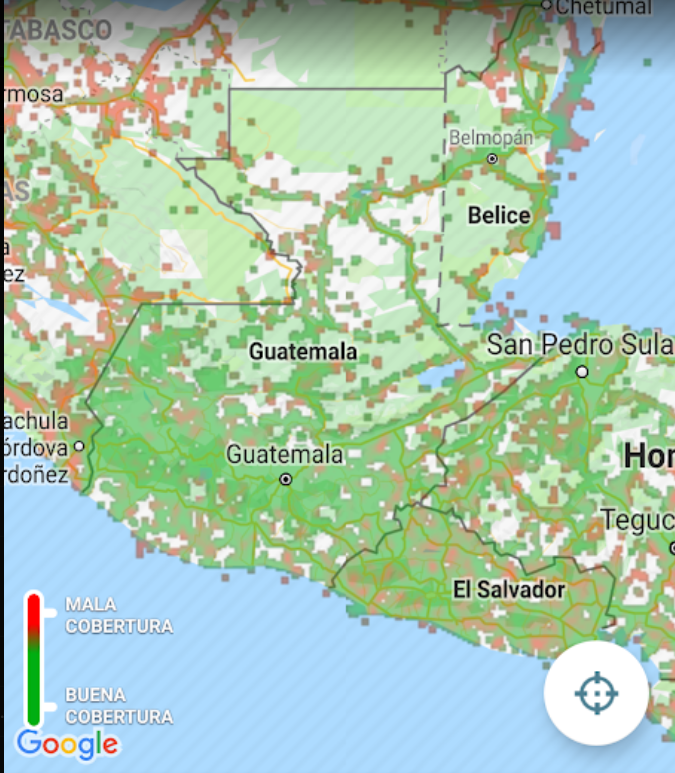
\includegraphics[height=0.75\textheight]{Docs/opensky}
    \caption{Cobertura celular de compañias Claro, Tigo y Movistar en bandas 2G, 3G y 4G.
    \emph{Fuente:www.opensignal.com}}
    \label{}
  \end{figure}
\end{frame}

\subsection{Tipos de instrumentación electrónica}
\begin{frame}{Tipos de instrumentación electrónica}
  \center
  Una tecnología solamente es tan buena como la persona que la aplica.
\end{frame}

\begin{frame}{Tipos de instrumentación electrónica}{Clasificación por precio}

  Según el costo de la instrumentación, esta la podemos catalogar en:
  \begin{itemize}
    \item Bajo
    \item Mediano
    \item Alto
    \item Experimental
  \end{itemize}
\end{frame}

\begin{frame}{Tipos de instrumentación electrónica}{Clasificación por precio}
  Según el costo de la instrumentación, esta la podemos catalogar en:
  \begin{itemize}
    \item \textbf{Bajo:}

      Pequeños agricultores y personas partículares
    \item \textbf{Mediano:}

      Cooperativas, Empresas privadas

    \item \textbf{Alto:}

      Comisiones departamentales, Estado de Guatemala.
    \item \textbf{Experimental:}

      Investigadores, Universidades
  \end{itemize}
\end{frame}



\end{document}
